\section{Max-min fairness example}

Under max-min fairness, the addition of flows to the network can \emph{increase} the throughput of some flows.

\expclass{abc}{mmfa}
To demonstrate this, we use a simple topology of three nodes with two directed edges:
\expline{abc}{the edge from A to B has a capacity of 1 unit},
and the \expline{abc}{the edge from B to C has a capacity of 1 unit}.

\expinstance{abc-one}{abc}
In the first experiment, we start the following flows: \expline{abc-one}{one from A to B} (path is A$\rightarrow$B), \expline{abc-one}{one from B to C} (path is B$\rightarrow$C), and \expline{abc-one}{one from A to C} (path is A$\rightarrow$B$\rightarrow$C).
This results in a max-min fair allocation of \expincludetext{abc-one}{flow-allocation-A-B.txt}, \expincludetext{abc-one}{flow-allocation-B-C.txt} and \expincludetext{abc-one}{flow-allocation-A-C.txt} for each type respectively.

\begin{center}
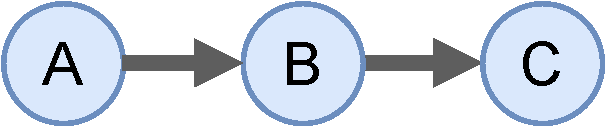
\includegraphics[width=4.5cm]{figures/topology-example.pdf}
\end{center}

\expinstance{abc-vary}{abc}
However, suppose that one would increase the number of flows from A to B. What would happen to the flow from B to C? In the second experiment, as before we start \expline{abc-vary}{one flow from B to C} and \expline{abc-vary}{one flow from A to C}. \expline{abc-vary}{We vary the number of flows from A to B between 1 and 4}. The addition of extra flows from A to B results in the flow from A to C being bottlenecked there, resulting in the flow from B to C being allocated more.

\begin{center}
\expincludegraphics[width=8cm]{abc-vary}
{num-flows-A-B-vs-flow-allocation-B-C.pdf}
\end{center}
